\documentclass{article}

\usepackage{graphicx}
\usepackage{hyperref}
\usepackage{bm}
\usepackage{float}
\restylefloat{table}

\usepackage{listings}
\usepackage{color}
\usepackage{amsmath}

\usepackage[margin=1.25in]{geometry}

\DeclareUnicodeCharacter{2212}{-}

\definecolor{dkgreen}{rgb}{0,0.6,0}
\definecolor{gray}{rgb}{0.5,0.5,0.5}
\definecolor{mauve}{rgb}{0.86,0.27,0.22}

\lstset{frame=tb,
  language=python,
  aboveskip=3mm,
  belowskip=3mm,
  showstringspaces=false,
  columns=flexible,
  basicstyle={\small\ttfamily},
  numbers=left,
  stepnumber=1,
  numberstyle=\tiny\color{gray},
  keywordstyle=\color{blue},
  commentstyle=\color{dkgreen},
  stringstyle=\color{mauve},
  breaklines=true,
  breakatwhitespace=true,
  tabsize=3
}

\title{CS5200: Final Exam} % Title of the assignment

\author{Matthew Whitesides\\ \texttt{mbwxd4@umsystem.edu}} % Author name and email address

\date{\today} % University, school and/or department name(s) and a date

%----------------------------------------------------------------------------------------

\begin{document}

  \maketitle % Print the title

  \textit{I, Matthew Whitesides, certify that all the material in this PDF file is my original work, that I did not discuss these questions with anyone other than my instructor, and that I did not copy work from anyone for this examination.}
 
  \begin{enumerate}
    \item \textbf{Hamiltonian Paths and Cycles}.
    
    Please refer to the following labled nodes version of the graph for some of the questions.\\
    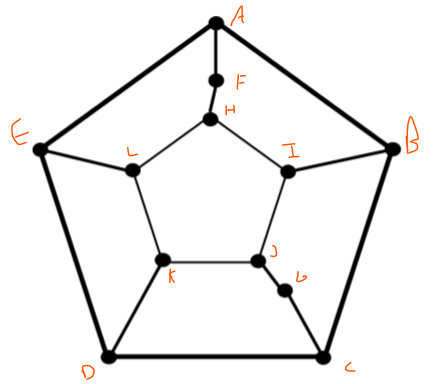
\includegraphics[scale=0.75]{1_Graph.png}

    \begin{enumerate}
        \item A Hamiltonian Path is defined as, "a graph path between two vertices of a graph that visits each vertex exactly once". Which yes this graph does have at least one. 
        
        For example the path in the labeled version above: 
        
        ${A \rightarrow F \rightarrow H \rightarrow I \rightarrow B \rightarrow C \rightarrow G \rightarrow J \rightarrow K \rightarrow D \rightarrow L}$ 
        
        would be a Hamiltonian Path.

        \item A Hamiltonian Cycle is defined as, " is a graph cycle (i.e., closed-loop) through a graph that visits each node exactly once.".
 
        Given a node has to be used once, each node that has a degree of 2 would have to have both of its edges used therefore edges (A,F),(F, H) and (J, G)(G, C) must be part of our cycle if one exists. 
        
        However, if we must include these four edges note that no matter which direction we attempt to get to vertices (A, H) and (J, G) we form a closed subcircuit. 
        See the graph below to demonstrate this note the blue are edges we know must be in there and red and orange are two possible paths to those edges and both form a closed-loop without including all the other vertices.

        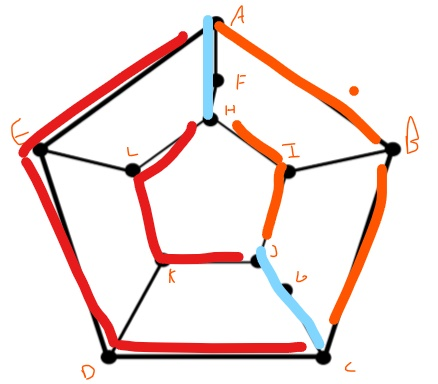
\includegraphics[scale=0.3]{1_Graph2.jpg}

        Therefore we know that this graph has no Hamiltonian cycle.

        \item
        \begin{itemize}          
          \item \textbf{The Problem.}
          \begin{itemize}
            \item We want to prove an n-dimensional cube contains a Hamiltonian Cycle. 
            \item An n-dimensional cube is defned as follows. It consists of the 2n vertices of the form $(a_0, a_1, ..., a_n)$ where each $a_i$ is either 0 or 1.
            \item Hamiltonian Cycle is defined as, " is a graph cycle (i.e., closed loop) through a graph that visits each node exactly once.".
            \item Our domain of n is any positive natual number in $n \ge 2$. As 0 would mean no edges or verticies and would be nothing, 1 would just be a line of two verticies which would not contain any cycles therefore not Hamiltonian, and a negitive numbers of edges does not make sense.
          \end{itemize}
          \item \textbf{Check the base case plus one.}
          \begin{itemize}
            \item Base case: $n = 2$: This is true as this is just a square with 4 verticies and 4 edges, and if you simply use every edge you have formed a Hamiltonian cycle.
            
            I.e. if you go though $(0,0) \rightarrow (0,1) \rightarrow (1,1) \rightarrow (1,0) \rightarrow returns\;to\;(0,0)$.
            \item $n = 3$: This would form a cube which we could represnt with the following graph (if you convert the letters to A = (0,0,0), B = (0,0,1).. etc:             
            
            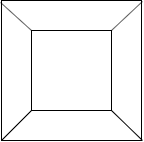
\includegraphics[scale=0.5]{cube.png}

            Which we can see has a Hamiltonian cycle if you follow the path:
            
            ${(A \rightarrow E \rightarrow F \rightarrow G \rightarrow H \rightarrow D \rightarrow C \rightarrow B \rightarrow returns\;to\;A)}$.
          \end{itemize}
          \item \textbf{The Inductive Hypothesis.}
          \begin{itemize}
            \item Lets assume using the induction Hypothesis that an (n - 1) dimensional cube does in fact contain a Hamiltonian Cycle.
            \item We can agree that cube n is essentailly cube (n - 1) with all adjecent edges connected to another (n - 1) cube.
            \item Lets define our n-dimensional cube as $C^n$.
            \item Therefore say for each vertex $v \in C^{n - 1}$ there is an adjecent vertex $v \in C'^{n - 1}$ that forms $C^n$.
            \item We can show this by our base cases of $n = 2$ is $(00, 01, 10, 11)$ then $n = 3$ is $(000, 001, 010, 011, 100, 101, 110, 111)$ .
            \item So we know that an n-cube contains $2^{n−1}n$ edges and $2^(n - 1) * 2$ verticies therefore we have an extra $2^{(-1 + n)} (-2 + n)$ edges connecting two adject $(n - 1)$ cubes. 
            \item We can also represent cube $n - 1$ within cube $n$ but adding a 0 in front of cube n's verticies (i.e. n = 2 is contained in (000, 001, 010, 011)) which we can call $v \in (0,1)^{n-1}$.
            \item And we can form a path from every edge $0_{v \in cube(n - 1)}$ like shown in the example above, except for the edge that goes though $0_n$ (or all zeros). This leaves an edge to connect to vertex $1_{v \in cube(n - 1)}$, then a path back to $0_n$.
            \item I.e. in the simple case n = 1 to n = 2. We have $v \in (0, 1)^1$ takes $0_{v \in cube(2 - 1)}$ or $00, 01$ connects those, then connects to $1_{v \in cube(2 - 1)}$ is $10, 11$ and finally back to $00$ to form the cycle.
            \item This using the Inductive Hypothesis can be scaled up to any $n \geq 2$. 
        \end{itemize}
        \item \textbf{Concluson.}        
        Therefore we have proven using the inductve Hypothesis that any n-dimensional cube where $n \ge 2$ does contain a Hamiltonian Cycle.
      \end{itemize}
    \end{enumerate}

    \item \textbf{General Graph Theory}.
    \begin{enumerate}
        \item \textbf{(Max Flow / Min Cut):}
        
        The minimal cut of the given transport network are simply the cut through the output of the input node S or the input to the sink node that cuts through edges $\{(g,a), (g, f), (g, s)\}$ or $\{(d,t), (g,t), (j,t)\}$. 
        As shown below:

        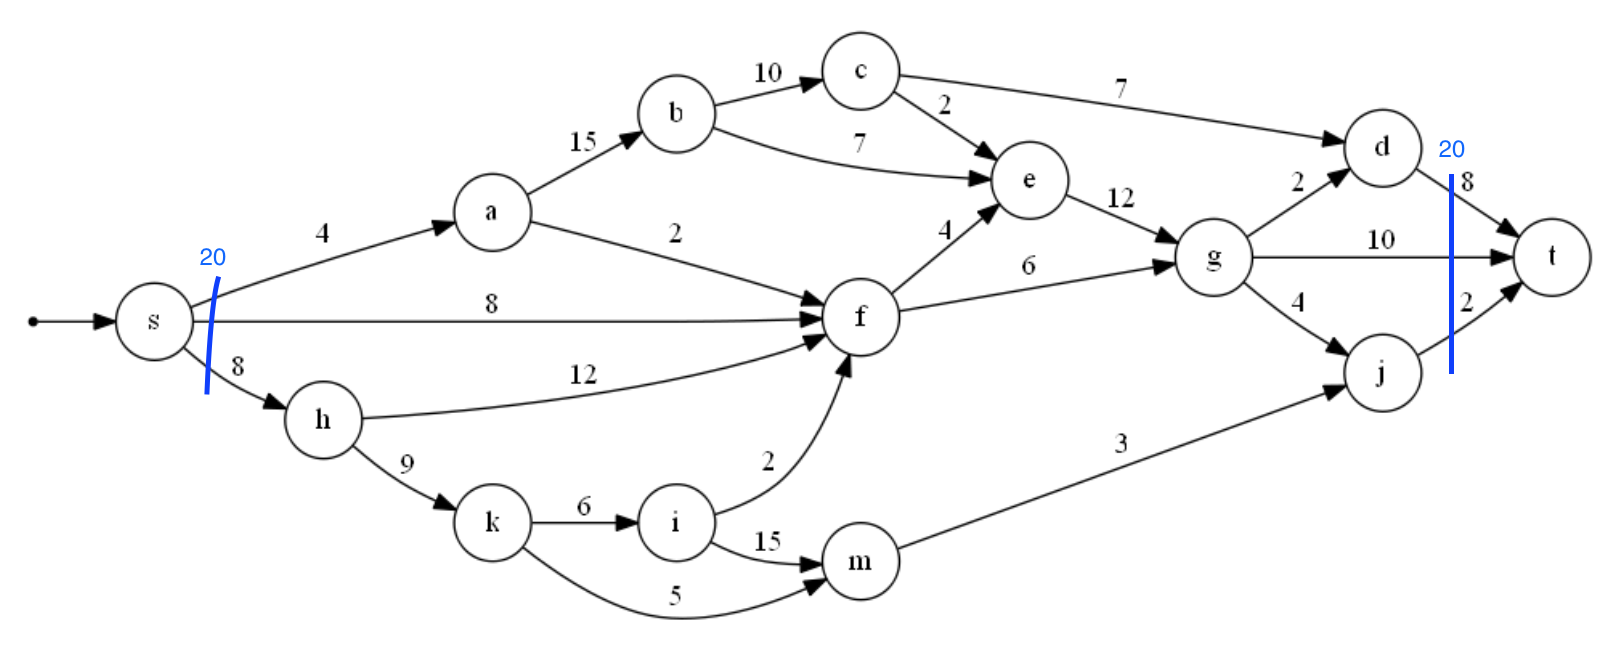
\includegraphics[scale=0.4]{2a}

        Therefore due the Max Flow / Min Cut theorm the maximal flow of the network is \bm{$f = 20$}.

        \item \textbf{(Handshaking):}
        
        Let's try a bit of a backword induction approach.
        
        If there are $N = 2$ people at the party then each person would have shaken hands with $(N - 1)$ person, e.g. the person other than John shook hands with one person which must be John.

        So if $Q(n)$ is out problem given $n$ people how many hands did John shake then $Q(2) = 1$.

        Now if $N = 3$ than we have John and two others which at most could have shaken hands with $(N - 1)$ person so the other handshakes would be $(N - 1), (N - 2)$ or $(2),(1)$.

        \item \textbf{(Vertex Degrees):}
        
        We want to prove every graph with $n \geq 2$ nodes must have at least two verticies having the same degree. \\
                
        First lets start with the possible degrees any given vertex can have in the graph with $n = num\;verticies$, then the range of possible degrees a vertex can have is $[1, n - 1]$. \\
        
        Therefore since the number of available options for $n$ verticies is $n - 1$ in the worst case we have at least one vertex that would have to share a degree with another one, since $n > (n - 1)$. \\
    
        Now if we take any gaph that contatins just a single pair of verticies we have a range of just $[1,1]$ possible degrees for each vertex. Therefore using the above proof the only degrees avaialbe to each vertex is a degree of 1. Just like a graph of $(A)-(B)$.

        \item \textbf{Connectedness:}
        
        To prove that $G'$ is connected when $G$ is disconnected let's start off saying that $G$ is disconnected. We just need to prove that $G'$ is connected.

        Lets say $(u, v) \notin G$ i.e. $(u, v)$ are a vertex edge pair that does not exsit in graph $G$, that means by definition that $(u, v) \in G'$ or $(u, v)$ are in $G$.
       
        Now since $G$ is disconnected into multiple subgraphs any edge $(u, v) \in G$ are part of a subgraph, therefore any edge $(u', v')$ that would connect two vertices in disconnect subgraphs must exist in $G'$.
       
        Finally, since $G$ is disconnected there is always an edge that does not exist from $v$ to any other $component\;subgraphs \in G$ meaning in the inverse $G'$ there must exist a vertex edge from each vertex in one subgraph to the other component subgraph(s).
       
        I.e. if you take two component subgraphs edges $G = {(A)}, {(B,C)}$ must become $G' = {(A,B),(A,C)}$.

        \item \textbf{Chess:}
        
        First, let's establish the number of possible moves a Knight can have. When it's free in every direction it has 6 possible moves when it's is in it's starting position or up against one wall there are 3, possible moves, and when it's in a corner there are 2 possible moves.

        Therefore we can create and $8*8$ or $64$ node graph with each node having a degree equal to the valid possible moves for that node and connected to the nodes where the knight would end up if doing those moves. Once we have that graph we would look for a Eulerian path or a path that goes through each node exactly once.
       
        However even we know that by definition a Eulerian path "is necessary that zero or two vertices have an odd degree;", which our nodes that have a degree of 3 where the knights up against the walls are greater than 2 as there's 4 walls and multiple positions on the walls.
       
        Therefore we know we cannot form a path in our graph that hits each node exactly once and thus the knight cannot move and hit each move exactly once.

        \item \textbf{Two Coloring:}
        
        A graph is two colorable if it is a Bipartite graph and by definition of a Bipartite graph, "a bipartite graph is a graph that does not contain any odd-length cycles.". 

        Now unfortunately since we have an even number of vertices with an odd number of edges there must be at least one vertex that creates an odd lengthed cycle. 
       
        Therefore we can not make a planar graph with 17 edges, and 10 vertices that can be 2-colored.
    \end{enumerate}

    \item \textbf{NP Complete Problems}.
    
    Note: Anytime I'm referencing the "book" I am referring to, "Introduction to Algorithms, 3rd Edition (The MIT Press) 3rd Edition by Thomas H. Cormen".
 
    \begin{enumerate}
      \item This particular problem is closely related to the "Circuit Satisfiability" problem in the book on p.1070 (see the book for full proof). Which is an \textbf{NP-Complete} problem on weather any given inputs in a circuit can produce a true output.
      You can pretty easily tell this problem in NP by simply taking a given solution and running it through the circuit to verify the faulty gate gives the same value no matter then input. 
      However, we know this type of problem is NP-Hard this proof essentially boils down to there's a polynomial-time number of input elements for every state in the circuit so even if a polynomial-time algorithm existed to verify one state each state would require a separate polynomial-time language. 
      
      \item I believe this problem is \textbf{NP-Complete}, if each node in a graph has a degree of two or less then it's essentially just a path with one in and one out edge for each node which is exactly what a "Hamiltonian Path" is, which is known to be NP-Complete, see book chapter 34.2 for proof.
      This problem is in NP as we can simply test in O(n) linear time if each node does have a degree of two or less. Also, this problem is closely related to the "Hamiltonian Cycle" problem which is NP-Complete which is just a Hamiltonian Path that ends at the same point it began. 
      Also, it's related to the "Circuit Satisfiability" problem we discussed in the previous question.
    
      \item We know that a minimum weight spanning tree (MST) can be found in \textbf{Polynomial Time} see book p.624 for an example of an O(E lg V) algorithm, and all we have to do once we have the MST is check if the total weight is less than some number K and you have your answer. 
      Therefore the problem is not NP-Hard and not NP-Complete. 
    
      \item Since we're not looking for the optimal scheduling solution we are just looking to see if we can schedule tasks under some constant time I call this solvable in \textbf{Polynomial Time} see book p.443 for an example of a task-scheduling solution. 
      Once we've found a minimum scheduling time we just need to check if it is under the given completion deadline. 
    
      \item First we can tell this problem is in NP easily by checking if our solution has each subset of vertices in $V_i \leq K$ and sum of weights of edges $V_i, V_j \leq J$ in at most $O(n^2)$ time. However, we are given Vertices, Edges, the sum of vertices, and the sum of edges.
      This is similar to the "Clique" problem, see book p.1087 with an added layer of complexity and that problem has been proven to be \textbf{NP-Complete}.      
    \end{enumerate}

    \item \textbf{Red-Black Trees, B-Trees, and Binary Search Trees}.
    
    \begin{enumerate}
      \item Below is an implemenation of a Red-Black Tree based on the algorithm in the book on p.315. Code is also avaialbe in the zip file in a file named 4a.py.
      
      \begin{lstlisting}
class Node():
    def __init__(self, key, left, right, color):
        self.key = key
        self.p = None
        self.left = left
        self.right = right
        self.color = color

class RBTree():
    def __init__(self):
        self.NIL = Node(0, None, None, "BLACK")
        self.root = self.NIL
        
    def print_tree(self):
        self.print_util(self.root, "", True)

    def print_util(self, node, tab, rightmost):
        if node != self.NIL:
            print(tab, end = "")            
            
            if rightmost:
                print("Right:", end = "")
            else:
                print("Left:", end = "")
            tab += "  "
                
            print("(" + str(node.key), node.color + ")")
            
            self.print_util(node.left, tab, False)
            self.print_util(node.right, tab, True)
    
    def get_height(self):
        return self.get_height_util(self.root, 0)
    
    def get_height_util(self, node, height):
        if node != self.NIL:
            height = self.get_height_util(node.right, height + 1)
        return height
        
    def rb_insert(self, z):
        z = Node(z, self.NIL, self.NIL, "RED")

        y = None
        x = self.root

        while x != self.NIL:
            y = x
            if z.key < x.key:
                x = x.left
            else:
                x = x.right

        z.p = y
        if y == None:
            self.root = z
        elif z.key < y.key:
            y.left = z
        else:
            y.right = z

        if z.p == None:
            z.color = "BLACK"
            return

        if z.p.p == None:
            return

        self.rb_insert_fixup(z)

    def rb_insert_fixup(self, z):
        while z.p.color == "RED":
            if z.p == z.p.p.right:
                u = z.p.p.left
                if u.color == "RED":
                    u.color = "BLACK"
                    z.p.color = "BLACK"
                    z.p.p.color = "RED"
                    z = z.p.p
                else:
                    if z == z.p.left:
                        z = z.p
                        self.right_rotate(z)

                    z.p.color = "BLACK"
                    z.p.p.color = "RED"
                    self.left_rotate(z.p.p)
            else:
                u = z.p.p.right

                if u.color == "RED":
                    u.color = "BLACK"
                    z.p.color = "BLACK"
                    z.p.p.color = "RED"
                    z = z.p.p
                else:
                    if z == z.p.right:
                        z = z.p
                        self.left_rotate(z)

                    z.p.color = "BLACK"
                    z.p.p.color = "RED"
                    self.right_rotate(z.p.p)

            if z == self.root:
                break

        self.root.color = "BLACK"

    def right_rotate(self, x):
        y = x.left
        x.left = y.right
        if y.right != self.NIL:
            y.right.p = x

        y.p = x.p
        if x.p == None:
            self.root = y
        elif x == x.p.right:
            x.p.right = y
        else:
            x.p.left = y

        y.right = x
        x.p = y

    def left_rotate(self, x):
        y = x.right
        x.right = y.left
        if y.left != self.NIL:
            y.left.p = x

        y.p = x.p
        if x.p == None:
            self.root = y
        elif x == x.p.left:
            x.p.left = y
        else:
            x.p.right = y

        y.left = x
        x.p = y        
      \end{lstlisting}

      Test output based on the graph show in the book p. 314 figure 13.3.

      \begin{lstlisting}
tree = RBTree()
tree.rb_insert(7)
tree.rb_insert(4)
tree.rb_insert(11)
tree.rb_insert(3)
tree.rb_insert(6)
tree.rb_insert(9)
tree.rb_insert(18)
tree.rb_insert(2)
tree.rb_insert(14)
tree.rb_insert(19)
tree.rb_insert(12)
tree.rb_insert(17)
tree.rb_insert(22)
tree.rb_insert(20)

print("RBTree Height:", tree.get_height())
tree.print_tree()       

# Output:
# RBTree Height: 5
# Right:(7 BLACK)
#   Left:(4 BLACK)
#     Left:(3 BLACK)
#       Left:(2 RED)
#     Right:(6 BLACK)
#   Right:(11 BLACK)
#     Left:(9 BLACK)
#     Right:(18 RED)
#       Left:(14 BLACK)
#         Left:(12 RED)
#         Right:(17 RED)
#       Right:(20 BLACK)
#         Left:(19 RED)
#         Right:(22 RED)
      \end{lstlisting}


      \item Below is the code used to generate 10 files of 10,000 random integers. See Zip file for all data files and 4b.py for full implemenation and code of the analysis below.
      
      \begin{lstlisting}
import random
import time
import statistics

for i in range(10):
    file_name = "Data{0}.txt".format(str(i))
    rn = [random.randint(1,10000) for i in range(10000)]
    f = open(file_name, "w+")
    for r in rn: 
        f.write(str(r) + "\n")

f.close()

for i in range(10):
  file_name = "Data{0}.txt".format(str(i))
  with open(file_name) as f:
      data_str = f.readlines()
  data.append([int(x.strip()) for x in data_str])

print(len(data))

# Output:
# 10
      \end{lstlisting}

      Below is the analysis of the RB Tree algorithm implementated above, see 4b.py for full code. 

      \begin{lstlisting}
heights = []
times = []

for i in range(10):
    start = time.time()
    
    tree = RBTree()
    for value in data[i]:
        tree.rb_insert(value)
    
    end = time.time()
    
    heights.append(tree.get_height())
    times.append(end - start)

    
print("RBTrees Heights:", str(heights))
print("RBTrees Times:", str(times))
print("")
print("RBTrees Heights Mean:", statistics.mean(heights))
print("RBTrees Heights median:", statistics.median(heights))
print("RBTrees Heights Standard Dev:", statistics.stdev(heights))
print("")
print("RBTrees Times Mean:", statistics.mean(times))
print("RBTrees Times median:", statistics.median(times))
print("RBTrees Times Standard Dev:", statistics.stdev(times))

# Output:
# RBTrees Heights: [14, 13, 14, 13, 15, 14, 14, 13, 15, 12]
# RBTrees Times: [0.07790899276733398, 0.1125800609588623, 0.07030510902404785, 0.06880617141723633, 0.06974482536315918, 0.06842374801635742, 0.12203192710876465, 0.06870102882385254, 0.06848478317260742, 0.0690760612487793]

# RBTrees Heights Mean: 13.7
# RBTrees Heights median: 14.0
# RBTrees Heights Standard Dev: 0.9486832980505138

# RBTrees Times Mean: 0.0796062707901001
# RBTrees Times median: 0.06941044330596924
# RBTrees Times Standard Dev: 0.02019085514989934
      \end{lstlisting}

      Next is my analysis of my BST algorihm from Prelim2, see 4b\_BST.py for full code.

    \begin{lstlisting}
class Node: 
    def __init__(self, v): 
        self.key = v 
        self.left = None
        self.right = None
                
def tree_insert(T, z): 
    y = None
    x = T
    while x:
        y = x
        if z.key < x.key:
            x = x.left
        else: x = x.right
    if y is None:
        T = z
    elif z.key < y.key:
        y.left = z
    else: y.right = z
                
def inorder_traversal(T): 
    if T: 
        inorder_traversal(T.left) 
        print(T.key, end=", ") 
        inorder_traversal(T.right)
        
def get_height(T):
    return get_height_util(T, 0)

def get_height_util(T, height):
    if T:
        height = get_height_util(T.left, height + 1)
    return height
    \end{lstlisting}

    BST analysis.

    \begin{lstlisting}
heights = []
times = []

for i in range(10):
    start = time.time()
    
    tree = Node(10000)
    for value in data[i]:
        tree_insert(tree, Node(value))
    
    end = time.time()
    
    heights.append(get_height(tree))
    times.append(end - start)

    
print("BST Heights:", str(heights))
print("BST Times:", str(times))
print("")
print("BST heights Mean:", statistics.mean(heights))
print("BST heights median:", statistics.median(heights))
print("BST heights Standard Dev:", statistics.stdev(heights))
print("")
print("BST Times Mean:", statistics.mean(times))
print("BST Times median:", statistics.median(times))
print("BST Times Standard Dev:", statistics.stdev(times))

# Output:
# BST Heights: [8, 10, 12, 14, 7, 10, 11, 10, 4, 12]
# BST Times: [0.04905128479003906, 0.04745912551879883, 0.04601430892944336, 0.06760406494140625, 0.04880189895629883, 0.04637598991394043, 0.04508614540100098, 0.04470682144165039, 0.07152700424194336, 0.048017024993896484]

# BST heights Mean: 9.8
# BST heights median: 10.0
# BST heights Standard Dev: 2.859681411936962

# BST Times Mean: 0.0514643669128418
# BST Times median: 0.047738075256347656
# BST Times Standard Dev: 0.009694087189213559
    \end{lstlisting}

    Finally is my analysis of my B-Tree algorihm from Prelim2, see 4b\_BTree.py for full code.

    \begin{lstlisting}
class Node(object):
    def __init__(self):
        self.leaf = False
        self.keys = []
        self.c    = []
        
    def print_node(self):
        if self.leaf:
            return "Leaf node:{}".format(self.keys)
        return "Node: {}\nChildren: {}\n".format(self.keys, [child.print_node() for child in self.c])

class BTree():
    def b_tree_create(self, t):
        x = Node()
        x.leaf = True
        self.t = t
        self.root = x
        
    def b_tree_split_child(self, x, i):
        z = Node()
        y = x.c[i]
        z.leaf = y.leaf
        t = self.t
        x.c.insert(i + 1, z)        
        x.keys.insert(i, y.keys[t - 1])  
        
        for j in range(t - 1):
            if len(z.keys) < t - 1:
                z.keys.append(0)
            z.keys[j] = y.keys[j  + t]
        y.keys = y.keys[0: (t - 1)]
        
        if not y.leaf:
            z.keys = y.keys[t: (2*t - 1)]
            y.keys = y.keys[0: (t-1)]

    def b_tree_insert(self, k):
        r = self.root
        if len(r.keys) == (2 * self.t) - 1:
            s = Node()
            self.root = s
            s.c.insert(0, r)
            self.b_tree_split_child(s, 0)  
            self.b_tree_insert_nonfull(s, k)
        else: self.b_tree_insert_nonfull(r, k)
    
    def b_tree_insert_nonfull(self, x, k):
        i = len(x.keys) - 1
        if x.leaf or len(x.c) is 0:
            x.keys.insert(len(x.keys), 0)
            while i >= 0 and k < x.keys[i]:
                x.keys[i + 1] = x.keys[i]
                i = i - 1
            x.keys[i + 1] = k
        else: 
            while i >= 0 and k < x.keys[i]:
                i = i - 1            
            i = i + 1
            if len(x.c[i].keys) == (2 * self.t) - 1:
                self.b_tree_split_child(x, i)
                if k > x.keys[i]:
                    i = i + 1
            self.b_tree_insert_nonfull(x.c[i], k) 
    
    def b_tree_delete(self, k):
        (n, i) = self.find(k)
        if n is None:
            return None
        
        if n.leaf:
            del n.keys[i]
        else:
            k = n.keys[i]
            if len(n.c[i]) >= self.t:
                pred = n.c[i]
                while not curr.leaf:
                    pred = curr.c[len(curr.c) - 1]
                n.keys[i] = pred
                b_tree_delete(pred)
                
            elif len(n.c[i + 1]) >= self.t:
                succ = n.c[i + 1]
                while not curr.leaf:
                    succ = succ.c[0]
                n.keys[i] = succ
                b_tree_delete(succ)
    
    def find(self, k, x = None):
        if isinstance(x, Node):
            i = 0            
            while i < len(x.keys) and k > x.keys[i]:
                i = i + 1
            if i < len(x.keys) and k == x.keys[i]: return (x, i)
            elif x.leaf: return (None, 0)
            else: return self.find(k, x.c[i])
        else: return self.find(k, self.root)
    
    def print_tree(self):
        out = self.root.print_node()
        out += '\n'.join([child.print_node() for child in self.root.c])
        return out
    
    def get_height(self):
        return self.get_height_util(0)

    def get_height_util(self, height):
        height += 1
        height = len([child.print_node() for child in self.root.c])
        return height      
    \end{lstlisting}

    Analysis for B-Tree's:

    \begin{lstlisting}
heights = []
times = []

for i in range(10):
    start = time.time()
    
    tree = BTree()
    tree.b_tree_create(1000)
    for value in data[i]:
        tree.b_tree_insert(value)
    
    end = time.time()
    
    heights.append(tree.get_height())
    times.append(end - start)

    
print("B-Tree Heights:", str(heights))
print("B-Tree Times:", str(times))
print("")
print("B-Tree heights Mean:", statistics.mean(heights))
print("B-Tree heights median:", statistics.median(heights))
print("B-Tree heights Standard Dev:", statistics.stdev(heights))
print("")
print("B-Tree Times Mean:", statistics.mean(times))
print("B-Tree Times median:", statistics.median(times))
print("B-Tree Times Standard Dev:", statistics.stdev(times))     

# Output:
# B-Tree Heights: [8, 8, 8, 8, 8, 8, 8, 8, 8, 8]
# B-Tree Times: [2.26718807220459, 2.235520839691162, 2.2249579429626465, 2.3519208431243896, 2.4345662593841553, 2.302553176879883, 2.6907920837402344, 2.6656839847564697, 2.4060938358306885, 2.428806781768799]

# B-Tree heights Mean: 8
# B-Tree heights median: 8.0
# B-Tree heights Standard Dev: 0.0

# B-Tree Times Mean: 2.4008083820343016
# B-Tree Times median: 2.379007339477539
# B-Tree Times Standard Dev: 0.1647701717343564
    \end{lstlisting}

    Therefore our final analysis is the following. Intresting however B-Trees are heavily dependent on the initial level set for them to create off of this would probably need to be tweaked.

    \begin{lstlisting}      
RBTrees Heights Mean: 13.7
RBTrees Heights median: 14.0
RBTrees Heights Standard Dev: 0.9486832980505138

RBTrees Times Mean: 0.0796062707901001
RBTrees Times median: 0.06941044330596924
RBTrees Times Standard Dev: 0.02019085514989934

BST heights Mean: 9.8
BST heights median: 10.0
BST heights Standard Dev: 2.859681411936962

BST Times Mean: 0.0514643669128418
BST Times median: 0.047738075256347656
BST Times Standard Dev: 0.009694087189213559

B-Tree heights Mean: 8
B-Tree heights median: 8.0
B-Tree heights Standard Dev: 0.0

B-Tree Times Mean: 2.4008083820343016
B-Tree Times median: 2.379007339477539
B-Tree Times Standard Dev: 0.1647701717343564      
    \end{lstlisting}

    \end{enumerate}

    \item \textbf{More Graph Algorithms}.
    
    \item \textbf{GCD}.
    
    \begin{enumerate}
        \item Lets say:
        
        \[GCD(p, q) = d\]
        
        Then we can say:

        \[p = p'd\]
        \[q = q'd\]

        \item TODO
        \item TODO
        
        \item The following is an implemenation based upon the previous three defintions and the EXTENDED-EUCLID algorithm in the book chapter 31.2. Code also avaialbe in the zip file under 6.py.
        
        \begin{lstlisting}
def gcd(p, q):
    p = format(p, 'b')
    q = format(q, 'b')
    result = gcd_util(p, q)
    return int(result, 2)

def gcd_util(p, q):
    # Base Cases
    if p == q:
        return p

    if is_zero(p):
        return p

    if is_zero(q):
        return q

    # Proof 6a: If p is even divide by two.
    if is_even(p):
        if is_even(q):
            return shift_left(gcd_util(shift_right(p), shift_right(q)))
        else:
            return gcd_util(shift_right(p), q)

    # Proof 6b: If p is odd and q is even.
    if (is_even(q)):
        return gcd_util(p, shift_right(q))

    # Proof 6c: If p and q are both odd and p > q.
    if is_greater(p, q):
        return gcd_util(shift_right(minus(p, q)), q)

    return gcd_util(shift_right(minus(q, p)), p)

def is_zero(s):
    return s == len(s) * '0'

def is_even(s):
    return s[len(s) - 1] == '0'

# Multiply by two, by adding a zero to the end.
def shift_left(s):
    return s + '0'

# Divide by two, by removing the last char.
def shift_right(s):
    return s[: -1]

def is_greater(x, y):
    if len(x) > len(y):
        return True
    return int(x, 2) > int(y, 2)

def minus(x, y):
    return format(int(x, 2) - int(y, 2), 'b')            
        \end{lstlisting}

        Next is some tests based upon the built in math function for 100 random numbers between 0 and 10,000,000.

        \begin{lstlisting}
import math
import random

rand_nums = [(random.randrange(0, 10000000), random.randrange(0, 10000000)) for i in range(100)]

for n in rand_nums:
    my_gcd = gcd(n[0], n[1])
    math_gcd = math.gcd(n[0], n[1])
    valid = my_gcd == math_gcd
    s = "GCD({},{}) = {}: Valid = {}".format(str(n[0]), str(n[1]), str(my_gcd), str(valid))
    print(s)

# Output:
GCD(1538856,3119886) = 198: Valid = True
GCD(7914355,1511558) = 1: Valid = True
GCD(7689698,3196157) = 1: Valid = True
GCD(9215805,9153735) = 15: Valid = True
GCD(689520,6448224) = 48: Valid = True
GCD(1091935,8600069) = 1: Valid = True
GCD(6699525,3740816) = 1: Valid = True
GCD(8343132,1335031) = 1: Valid = True
GCD(5668326,6372101) = 1: Valid = True
GCD(507207,7191700) = 1: Valid = True
GCD(1657302,8695889) = 1: Valid = True
GCD(3895432,9300223) = 1: Valid = True
GCD(1447369,4070530) = 1: Valid = True
GCD(625554,7662878) = 2: Valid = True
GCD(4099520,9983340) = 20: Valid = True
GCD(4242430,8746934) = 2: Valid = True
GCD(4224013,9944584) = 1: Valid = True
GCD(7924562,8333583) = 1: Valid = True
GCD(3689938,7683761) = 1: Valid = True
GCD(2538929,5714762) = 1: Valid = True
GCD(7283602,6257603) = 1: Valid = True
GCD(6224831,3717497) = 1: Valid = True
GCD(9902804,5713719) = 1: Valid = True
GCD(3486538,444740) = 2: Valid = True
GCD(9727931,3666453) = 1: Valid = True
GCD(5103688,7288129) = 1: Valid = True
GCD(1813503,2072732) = 1: Valid = True
GCD(2335878,6392912) = 2: Valid = True
GCD(1346708,6402414) = 2: Valid = True
GCD(5094314,205662) = 2: Valid = True
GCD(6004650,5128461) = 3: Valid = True
GCD(9168461,9678714) = 1: Valid = True
GCD(2458709,4581295) = 1: Valid = True
GCD(8260594,8354852) = 2: Valid = True
GCD(8588868,6014742) = 6: Valid = True
GCD(9133893,3748095) = 9: Valid = True
GCD(2767474,8592140) = 2: Valid = True
GCD(2783352,1884924) = 12: Valid = True
GCD(1506689,8603835) = 1: Valid = True
GCD(972762,5818927) = 1: Valid = True
GCD(1469327,210559) = 1: Valid = True
GCD(4389611,5808938) = 1: Valid = True
GCD(4773064,9205376) = 8: Valid = True
GCD(9120320,5344503) = 1: Valid = True
GCD(3690248,7216206) = 2: Valid = True
GCD(5514667,1897652) = 1: Valid = True
GCD(9465515,520126) = 1: Valid = True
GCD(6947848,8186467) = 1: Valid = True
GCD(1520632,2273765) = 1: Valid = True
GCD(8056159,4056243) = 1: Valid = True
GCD(7370289,4497508) = 1: Valid = True
GCD(7926750,6743645) = 5: Valid = True
GCD(3834517,5254726) = 1: Valid = True
GCD(2354774,2429083) = 1: Valid = True
GCD(3100935,3779216) = 1: Valid = True
GCD(9000615,4923537) = 3: Valid = True
GCD(8504032,4515543) = 1: Valid = True
GCD(9668345,9586247) = 1: Valid = True
GCD(3410580,9316504) = 4: Valid = True
GCD(9976159,2307393) = 1: Valid = True
GCD(334049,561823) = 1: Valid = True
GCD(4302445,1028250) = 5: Valid = True
GCD(8887907,5956705) = 1: Valid = True
GCD(774851,7782759) = 29: Valid = True
GCD(143844,7501340) = 4: Valid = True
GCD(2954894,8403757) = 1: Valid = True
GCD(4775893,4355683) = 1: Valid = True
GCD(4349212,8702977) = 1: Valid = True
GCD(8748750,4768746) = 6: Valid = True
GCD(3654456,1339660) = 4: Valid = True
GCD(130625,4382430) = 5: Valid = True
GCD(7393393,8294257) = 1: Valid = True
GCD(74839,2065316) = 1: Valid = True
GCD(2836026,6028635) = 3: Valid = True
GCD(6656040,7303050) = 90: Valid = True
GCD(6582605,3174664) = 1: Valid = True
GCD(9037991,4158127) = 1: Valid = True
GCD(4374985,9406388) = 1: Valid = True
GCD(3431537,5710879) = 1: Valid = True
GCD(4522902,8356726) = 2: Valid = True
GCD(9645750,1487810) = 10: Valid = True
GCD(7797770,6749390) = 10: Valid = True
GCD(8849941,9409346) = 1: Valid = True
GCD(6701792,1346482) = 2: Valid = True
GCD(1297385,3483966) = 1: Valid = True
GCD(3011548,9145584) = 172: Valid = True
GCD(464411,8283354) = 1: Valid = True
GCD(2124342,4066508) = 2: Valid = True
GCD(3736756,8176411) = 1: Valid = True
GCD(34389,2818507) = 1: Valid = True
GCD(7083235,7095524) = 1: Valid = True
GCD(1535923,7422923) = 1: Valid = True
GCD(8946907,2019604) = 1: Valid = True
GCD(4951742,3698815) = 1: Valid = True
GCD(171714,7487361) = 3: Valid = True
GCD(9240535,5032304) = 1: Valid = True
GCD(6453503,5370161) = 1: Valid = True
GCD(9156934,2304982) = 2: Valid = True
GCD(9889135,3125602) = 1: Valid = True
GCD(9507098,4548646) = 2: Valid = True    
        \end{lstlisting}
    \end{enumerate}
  \end{enumerate}  % End of questions.
\end{document}
